\thispagestyle{fancy}
\vspace*{40 pt}

\section{\large{\MakeUppercase{Telas IHM alimentação}}}
Devido ao tamanho reduzido desta tela, não foi possível inserir todas as funcionalidades disponíveis na IHM da Corte e Vinco e do Empilhador.
 Porém um grande trabalho de UX foi realizado para que o operador pudesse realizar todas as tarefas necessárias para o ajuste da unidade mantendo
 o estilo e navegação da IHM das telas grandes. Na IHM da alimentação, o operador pode realizar apenas alguns ajustes da unidade e máquina e existem
 alguns ajustes que são realizados apenas por esta tela por questões de facilidade de acesso e de se tratar de ajustes que requerem visualização pois
 não possuem encoders para ajuste automático.
 
\subsection{\small{Tela principal}}\label{ihmAlimentacaoTelaPrincipal}

Na tela principal possui os botões de acesso as telas de ajustes e comandos da unidade por meio do menu esquerdo superior, também é possível acessar
os alarmes por meio do botão esquerdo inferior, estes menus permanecem iguais em todas as telas. Além disso, é possível visualizar algumas informações 
sobre o pedido atual, como o nome do pedido, a quantidade de caixas a serem produzidas, a quantidade de caixas produzidas, a quantidade de caixas
do pedido anterior e a quantidade de caixas produzidas por minuto (velocidade da máquina). Também é possível ajustar a velocidade da máquina clicando
sobre o campo de velocidade e utilizando o teclado numérico para inserir o valor desejado.


\subsection{\small Habilita alimentação de chapas}
\vspace*{\fill}
\begin{figure}[h]
    \centering
    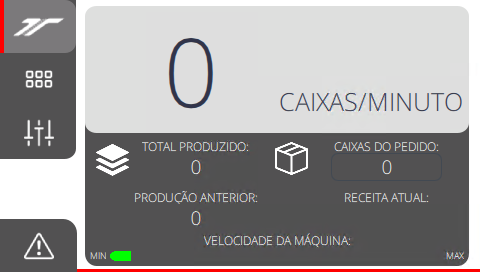
\includegraphics{src/imagesFlexo/11-IHMALM/e-1.png}
\end{figure}
\vspace*{\fill}

\newpage
\thispagestyle{fancy}
\vspace*{40 pt}
\subsection{\small Informações da máquina}
\vspace*{\fill}
\begin{figure}[h]
    \centering
    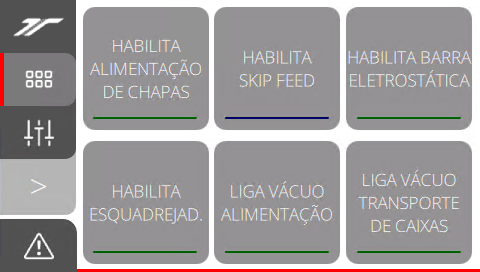
\includegraphics{src/imagesICV/11-KTP400-Feeder/2.png}
\end{figure}
\vspace*{\fill}

\newpage
\thispagestyle{fancy}
\vspace*{40 pt}
\subsection{\small Comandos da unidade}
\vspace*{\fill}
\begin{figure}
    \centering
    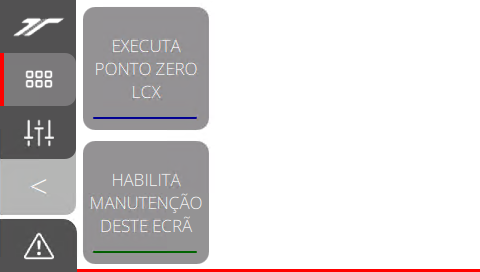
\includegraphics{src/imagesICV/11-KTP400-Feeder/3.png}
\end{figure}
\vspace*{\fill}

\newpage
\thispagestyle{fancy}
\vspace*{40 pt}
\subsection{\small Comandos da unidade}
\vspace*{\fill}
\begin{figure}[h]
    \centering
    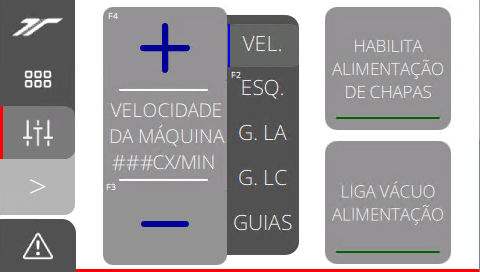
\includegraphics{src/imagesICV/11-KTP400-Feeder/4.png}
\end{figure}
\vspace*{\fill}

\newpage
\thispagestyle{fancy}
\vspace*{40 pt}
\subsection{\small Tela de alarmes}
\vspace*{\fill}
\begin{figure}[h]
    \centering
    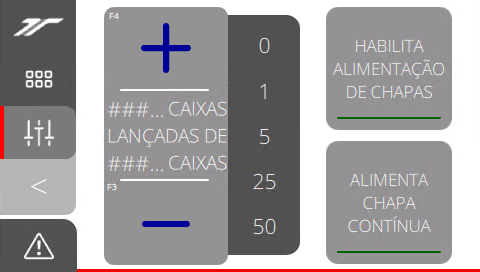
\includegraphics{src/imagesICV/11-KTP400-Feeder/10.png}
\end{figure}
\vspace*{\fill}
